\documentclass[tikz,border=6pt]{standalone}
\usetikzlibrary{arrows.meta,positioning}
\begin{document}
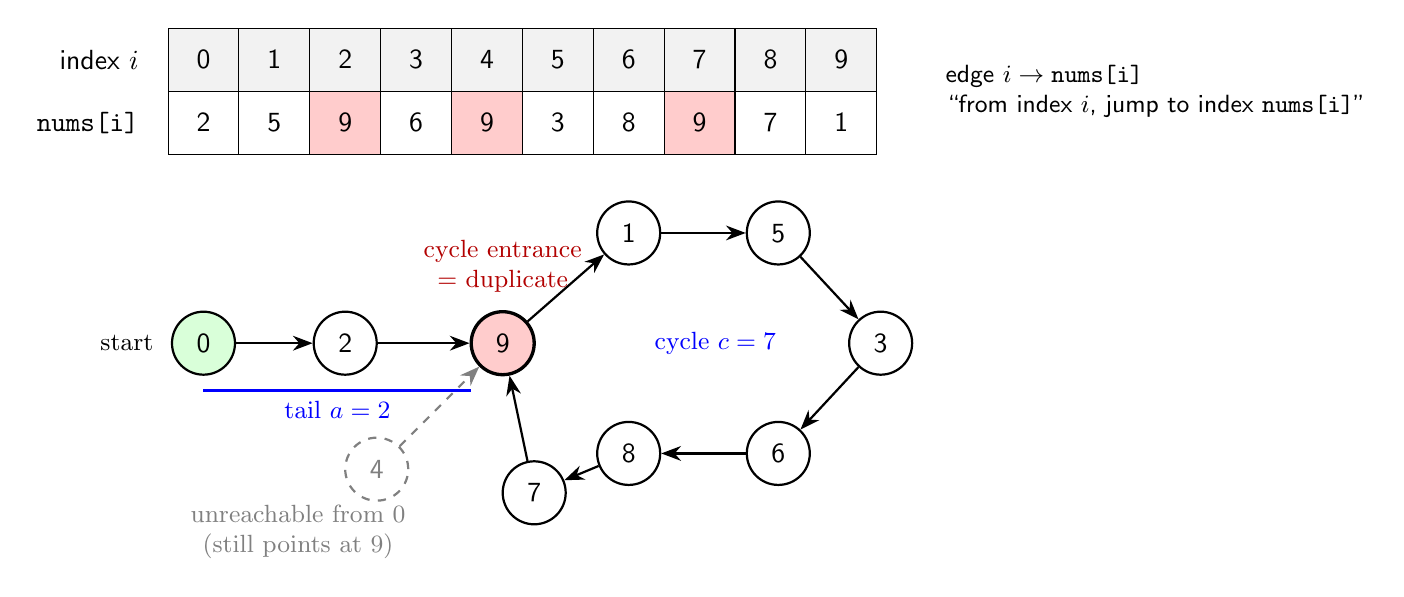
\begin{tikzpicture}[font=\sffamily,
  cell/.style={draw,minimum width=9mm,minimum height=8mm},
  node_/.style={circle,draw,thick,minimum size=8mm},
  ar/.style={-{Stealth[length=2.5mm]},thick}]
\node[anchor=east] at (-0.7,0) {index $i$};
\node[anchor=east] at (-0.7,-0.8) {\texttt{nums[i]}};
\foreach \v [count=\i from 0] in {2,5,9,6,9,3,8,9,7,1} {
  \node[cell,fill=gray!10] at (\i*0.9,0) {\i};
  \node[cell] (c\i) at (\i*0.9,-0.8) {\v};
}
\foreach \i in {2,4,7} \node[cell,fill=red!20] at (\i*0.9,-0.8) {9};
\node[align=left,anchor=west,font=\sffamily\small] at (9.3,-0.4) {edge $i \to \texttt{nums[i]}$\\ ``from index $i$, jump to index \texttt{nums[i]}''};
% graph
\begin{scope}[yshift=-3.6cm]
\node[node_,fill=green!15] (n0) at (0,0) {0};
\node[node_] (n2) at (1.8,0) {2};
\node[node_,fill=red!20,very thick] (n9) at (3.8,0) {9};
\node[node_] (n1) at (5.4,1.4) {1};
\node[node_] (n5) at (7.3,1.4) {5};
\node[node_] (n3) at (8.6,0) {3};
\node[node_] (n6) at (7.3,-1.4) {6};
\node[node_] (n8) at (5.4,-1.4) {8};
\node[node_] (n7) at (4.2,-1.9) {7};
\node[node_,dashed,gray] (n4) at (2.2,-1.6) {4};
\draw[ar] (n0)--(n2); \draw[ar] (n2)--(n9);
\draw[ar] (n9)--(n1); \draw[ar] (n1)--(n5); \draw[ar] (n5)--(n3); \draw[ar] (n3)--(n6);
\draw[ar] (n6)--(n8); \draw[ar] (n8)--(n7); \draw[ar] (n7)--(n9);
\draw[ar,dashed,gray] (n4)--(n9);
\node[left=1mm of n0,font=\small] {start};
\node[above=1mm of n9,font=\small,red!70!black,align=center] {cycle entrance\\= duplicate};
\draw[thick,blue] (0,-0.6)--(3.4,-0.6);
\node[blue,font=\small] at (1.7,-0.85) {tail $a=2$};
\node[blue,font=\small] at (6.5,0) {cycle $c=7$};
\node[gray,font=\small,align=center] at (1.2,-2.4) {unreachable from 0\\(still points at 9)};
\end{scope}
\end{tikzpicture}
\end{document}
